	\subsubsection{UC\theuccount-GL - Gitlab segnala la modifica di una issue al Producer Gitlab}
	\begin{figure}[H]
		\centering
		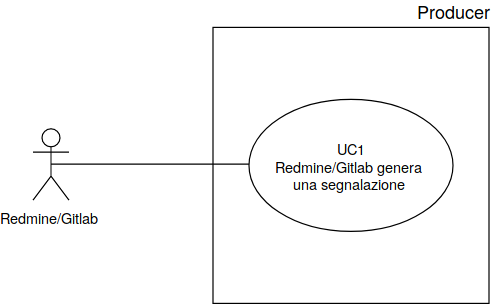
\includegraphics[width=0.7\textwidth]{img/UC1.png}\\
		\caption{UC\theuccount-GL - Gitlab segnala la modifica di una issue al Producer Gitlab}
	\end{figure}
	\begin{itemize}
		\item \textbf{Codice}: UC\theuccount-GL.
		\item \textbf{Titolo}: Gitlab segnala la modifica di una issue al Producer Gitlab.
		\item \textbf{Attori primari}: GitLab.
		\item \textbf{Descrizione}: il sistema qui è Producer GitLab ed è interno al sistema Butterfly. L'invio di una segnalazione avviene
		da parte di GitLab tramite webhook, quando una issue viene modificata.
		\item \textbf{Precondizione}: Viene modificata una issue già aperta su un
		progetto di GitLab e segnalata a \progetto.
		\item \textbf{Postcondizione}: il Producer GitLab riceve la segnalazione da GitLab.
		\item \textbf{Scenario principale}: 
		\begin{enumerate}
			\item GitLab procede all'invio della segnalazione di modifica issue al Producer GitLab
		\end{enumerate}
		
	\end{itemize}